\documentclass[12pt]{article}

% Language setting
\usepackage[utf8]{inputenc}
\usepackage[bulgarian]{babel}

% --------------------- Packages  --------------------
% Use biblatex
\usepackage{biblatex}
\addbibresource{bibliography.bib}
% Table thickness
\usepackage{ctable}
% Equations: SI units
\usepackage{siunitx}
% Approximately equal
\usepackage{amssymb}
% degrees symbol
\usepackage{gensymb}
% warning box
\usepackage{pifont,mdframed}
% Multiline math
\usepackage{amsmath}

\newenvironment{warning}
  {\par\begin{mdframed}[linewidth=2pt, linecolor=white]%
    \begin{list}{}{\leftmargin=1cm
                   \labelwidth=\leftmargin}\item[\Large\ding{43}]}
  {\end{list}\end{mdframed}\par}

% --------------------- Title  --------------------
\addbibresource{bibliography.bib}

\begin{document}

% Anfang der Titelseite________________________________________________________________________________
\begin{titlepage}
	\flushleft
% 	\begin{center}
	%{\scshape\Large Werkstoffe III \hspace{2.5cm} Laborbericht \hspace{2.5cm}HS 2022 \par}
	{\scshape\Large Протокол IV \hspace{2cm} Молекулна физика\par}
	\vspace{4cm}
	{\huge\bfseries Измерване на специфичен топлинен капацитет по метода на охлаждането\par}
	\vspace{1cm}
	{\LARGE\bfseries Лабораторно упражнение №3.10\par}
	\vspace{5cm}
    {\LARGE\bfseries Виолета Кабаджова, \par}
%   {\LARGE\bfseries Group: X\par}
    {\large\bfseries ККТФ, фак. номер: 3PH0600026\par}
	\vspace{1cm}
	
	{\large Физически Факултет, 
	
	Софийски Университет "Св. Климент Охридски"
	
	4 април 2023 г.\par}
	
\end{titlepage}

\section{Теоритична част}\label{sec:theoretical-part}
При охлаждането на нагрят образец в околната среда се отделя топлина през повърхността му, равна количествено на израза във формула \ref{eq:q-unit-surface}, където $Q$ е количеството топлина, $\alpha$ - коефициентът на топлоотдаване, $T$ - температурата на повърхността на образеца, $T_0$ - температурата на околната среда. Количеството топлина, отделено от цялата повърхност на едно тяло обаче, при малки геометрични размери е равно на количеството топлина, отделена от обема на това тяло, изразено чрез формула \ref{eq:q-volume}, където $c$ е специфичният топлинен капацитет, $\rho$ - плътността на изследвания образец, а $V$ - обемът му. Следователно бихме могли да приравним тези два израза, получавайки формула \ref{eq:1-to-3}.

\begin{equation}\label{eq:q-unit-surface}
    Q = \int_S \alpha(T - T_0)dS
\end{equation}

\begin{equation}\label{eq:q-volume}
    Q = c \rho \frac{dT}{dt}V
\end{equation}

\begin{equation}\label{eq:1-to-3}
    c \rho \frac{dT}{dt}V = \alpha(T - T_0)S
\end{equation}

Разполагайки с два образеца, параметрите на единия от които знаем, бихме могли да определим специфичния топлинен капацитет $c$ на даден метал без да се знае коефициента $\alpha$. Когато те са с еднаква форма и повърхност ($S_1$ = $S_2$) и са заглети до една и съща температура ($T_1$ = $T_2$), охлаждайки се в една и съща околна среда, то тогава се получава формула \ref{eq:divided}, откъдето следва работната формула \ref{eq:work-formula}.

\begin{equation}\label{eq:divided}
    \frac{c_1\rho_1(\frac{dT}{dt})_1V_1}{c_2\rho_2(\frac{dT}{dt})_2V_2} = \frac{c_1m_1(\frac{dT}{dt}_1)}{c_2m_2(\frac{dT}{dt})_2} = 1    
\end{equation}

\begin{equation}\label{eq:work-formula}
    c_1 = \frac{c_2m_2(\frac{dT}{dt})_2}{m_1(\frac{dT}{dt})_1}
\end{equation}


\section{Експериментална част}

\subsection{Експериментална установка}
\begin{figure}
    \centering
    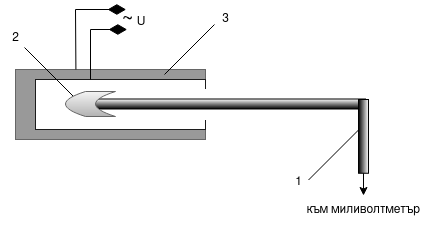
\includegraphics[width=0.8\textwidth]{images/setup.png}
    \caption{Схема на опитна постановка: 1 - термодвойка, 2 - метален образец, 3 - пещ}
    \label{fig:setup}
\end{figure} 

На фиг. \ref{fig:setup} е илюстрирана схема на опитната установка. Нагряването на образците се осъществява посредством пещ, а измерванаето на температурата - чрез термодвойка.

\subsection{Задача: Получаване на кривата на охлаждане $T_2(t)$ за еталонен меден образец и $T_1(t)$ за изследван железен образец}
На фиг. \ref{fig:T2-of-t} и \ref{fig:T1-of-t} са показани съответно графиките на охлаждане на медения (414 $\degree$C до 86 $\degree$C) и железния (419 $\degree$C до 86 $\degree$C) образец.

\subsection{Задача: Измерване скоростите на охлаждане при температура 300 $\degree $C за еталонния и изследвания образец}
Скоростта на охлаждане на образците определяме чрез разликата между петото и тринайсетото измерване (диапазона около 300 $\degree$C за двете криви: 300 $\pm$ 42 $\degree$C за $T_1$ и 300 $\pm$ 50 $\degree$C за $T_2$), разделено на разликата на времената за съответните измервания:

\begin{align*} 
    \left(\frac{dT}{dt}\right)_1 = \frac{T_{1-2} - T_{1-1}}{t_2 - t_1} = \frac{343 - 258}{(10 - 5)\cdot 15} = 0.807 \degree C / s\\
    \left(\frac{dT}{dt}\right)_2 = \frac{T_{2-2} - T_{2-1}}{t_2 - t_1} = \frac{355 - 256}{(10 - 5)\cdot 15} = 0.708 \degree C / s
\end{align*}

\begin{table}[h]
\begin{center}
\begin{tabular}{|l|l|l|} \hline
N &T_1, \degree C &T_2, \degree C \\ \hline
5 &343 &355 \\ \hline
6 &331 &336 \\ \hline
7 &324 &321 \\ \hline
8 &321 &309 \\ \hline
9 &307 &297 \\ \hline
10 &290 &285 \\ \hline
11 &283 &273 \\ \hline
12 &261 &263 \\ \hline
13 &258 &256 \\ \hline
\end{tabular}
\caption{\label{tbl:measurements}Измервания за медния и железния образец през време t=15$s$ в температурен диапазон около 300 $\degree$C}
\end{center}
\end{table}

Относителната графична грешка за $\left(\frac{dT}{dt}\right)$ определяме посредством формула \ref{eq:max-err-dTdt}, където $T^*_5$ и $T^*_{13}$ са стойностите на съответно петото и тринайстото измерване.

\begin{equation}\label{eq:max-err-dTdt}
    \frac{\Delta \left(\frac{dT}{dt}\right)}{\left(\frac{dT}{dt}\right)} = \frac{\Delta T^*_5 + \Delta T^*_{13}}{T^*_5 - T^*_{13}} + \frac{\Delta t_{13} + \Delta t_{5}}{t_{13} - t_{5}}
\end{equation}

\begin{figure}
    \centering
    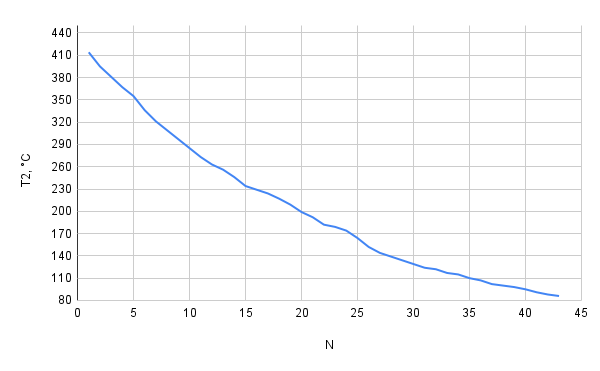
\includegraphics[width=0.8\textwidth]{images/chart-T2.png}
    \caption{\label{fig:T2-of-t}Крива на охлаждане $T_2(t)$ за меден образец}
\end{figure} 

\begin{figure}
    \centering
    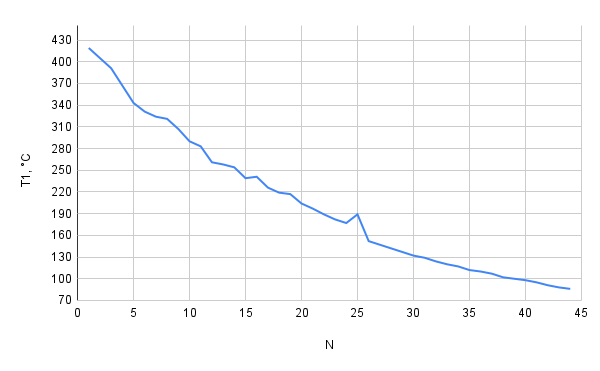
\includegraphics[width=0.8\textwidth]{images/chart-T1.png}
    \caption{\label{fig:T1-of-t}Крива на охлаждане $T_1(t)$ за железен образец}
\end{figure} 

\subsection{Задача 4: Измерване специфичния топлинен капацитет на изследвания метал}
Специфичния топлинен капацитет на желязото пресмятаме по формула \ref{eq:work-formula}, като получаваме $c_1 = 473 \pm 44 \frac{J}{kg.K}$

\end{document}
